\chapter{Methodology}

\section{Image Preprocessing}

\begin{figure}[H]
    \centering
    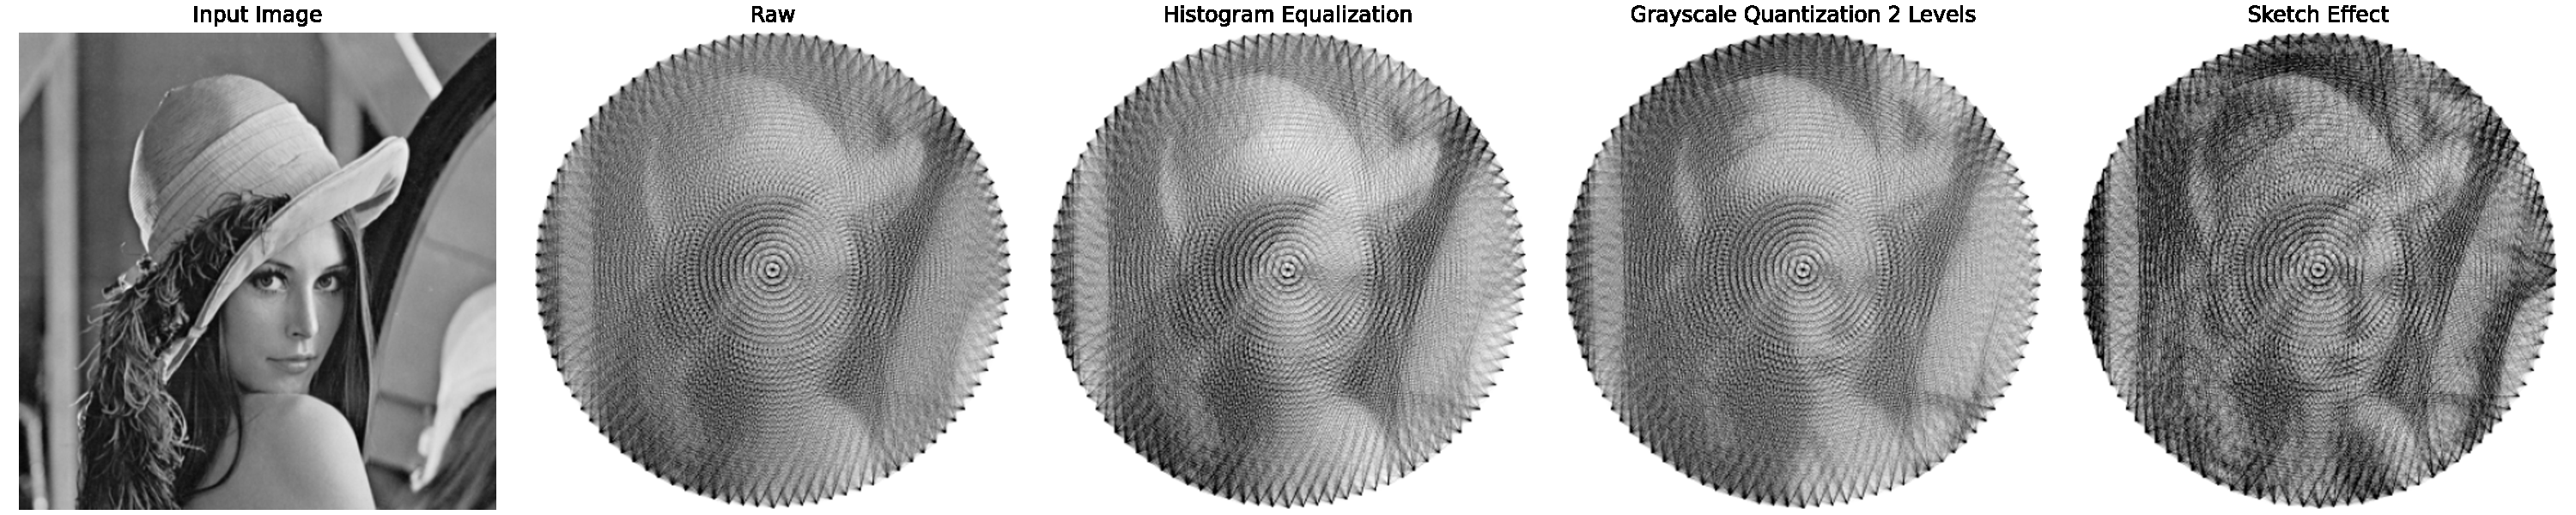
\includegraphics[width=\linewidth]{images/preprocess/preprocessed_results.pdf}
    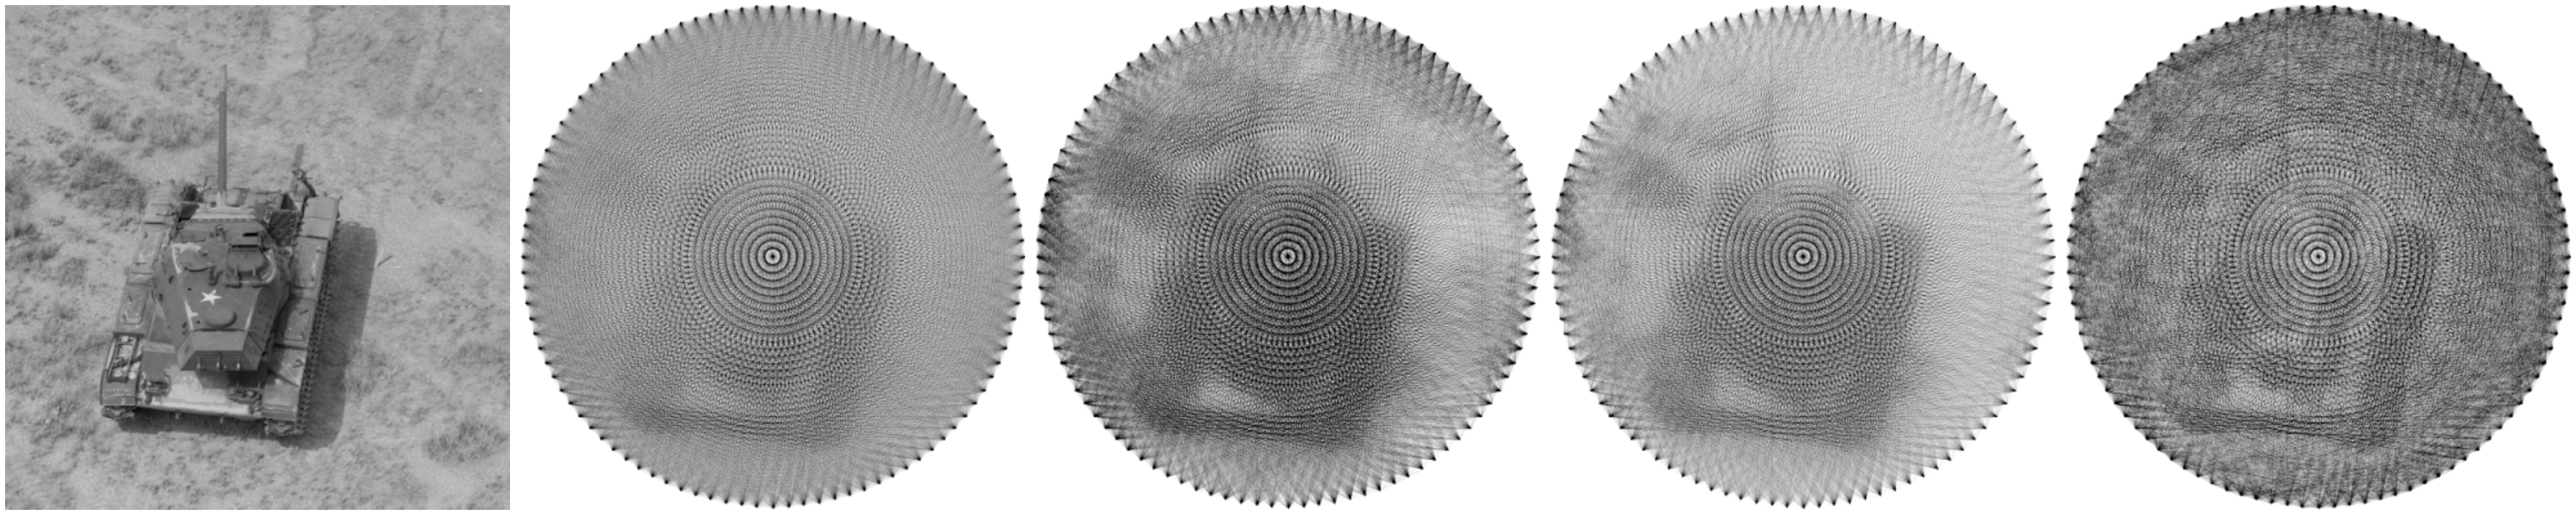
\includegraphics[width=\linewidth]{images/preprocess/preprocessed_results_tank.pdf}
    \caption{Comparative analysis of results using different preprocessing methods.}
    \label{fig:preprocess_results}
\end{figure}

Different preprocessing methods were tried, and a comparative analysis was conducted to determine the best subjective image quality. The raw result is very gray, making it somewhat difficult to distinguish details. Histogram Equalization\footnote{Details about the histogram equalization method can be found on \href{https://docs.opencv.org/4.x/d4/d1b/tutorial_histogram_equalization.html}{OpenCV: Histogram Equalization}} adds a touch of contrast. The sketch effect\footnote{Details about the sketch effect method can be found on \href{https://medium.com/@Kavya2099/image-to-pencil-sketch-using-opencv-ec3568443c5e}{8 Steps To Convert Image To Pencil Sketch Using OpenCV}} adds a lot of background noise, the image becomes darker and contains significantly more detail. Grayscale quantization\footnote{Details about the grayscale quantization method can be found on \href{https://en.wikipedia.org/wiki/Quantization_(image_processing)\#Grayscale_quantization}{Quantization (image processing)}} using two levels of quantization seems to strike a perfect balance between the two.

The final method we decided to use is Histogram Equalization because it is not too aggressive and effectively brings images to consistent tonality levels.

\section{Supersampling} \label{sec:supersampling}

In the case of a binary \(x\) resulting vector, the rendered lines are too thick, making the image appear overly dark, even when only a limited number of lines are drawn. In reality, human perception interprets the density of string intersections as varying shades of gray, not absolute black.

This formulation \ref{eq:least_squares} operates at low resolution. However, to more accurately capture the visual effect of overlapping strings, we employ supersampling, a technique that involves computing in a higher resolution and then downsampling the result. Specifically, we upscale the matrix \(A\), denoted as \(\bar{A}\), compute the product \(\bar{A}x\), and then apply a downsampling operator \(D : \left[ 0, 1\right] ^ {\sigma^2m^2} \rightarrow \left[ 0, 1\right] ^ {m^2}\), which averages non-overlapping blocks of size \(\sigma \times \sigma\), to bring the result back to the original resolution before comparing it to the target image \(b\). The new objective becomes:

\begin{equation}
\label{eq:supersampling}
\min{\| D(\bar{A} x) - b \|^2}
\end{equation}

\section{Least Squares (LS)}

The simplest method to solve Equation \ref{eq:least_squares} is by using a least squares approach. It minimizes the following function:

\begin{equation}
\min_{x}{||Ax - b||^2}
\end{equation}

This involves choosing the vector \(x\) such that the \(l^2\) norm between the linear combination of lines and the input image is minimized.

There are two ways to represent the matrix \(A\) in memory. The first is using a dense matrix, which explicitly stores each element in memory. This results in a computation time of approximately \(2.75\) minutes and \(6GB\) of memory usage for \(N=100\). 

However, considering the structure of the matrix \(A\), where each column vector represents a flattened image with only one line drawn, it is evident that the matrix is very sparse. 

\begin{figure}[H]
    \centering
    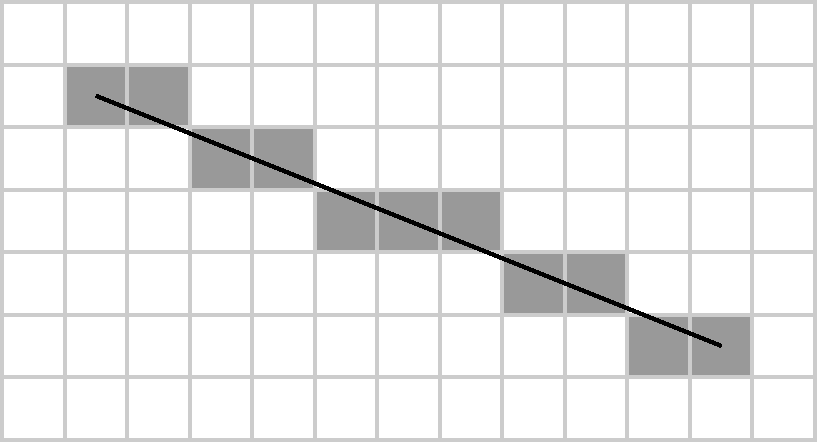
\includegraphics[width=0.33\linewidth]{images/bresenham.pdf}
    \caption{Illustration demonstrating the Bresenham line rendering method.}
    \label{fig:bresenham}
\end{figure}

Since \(A_i \in \mathbb{R^{m^2}}\),  and the maximum number of pixels a line can cover in a matrix of shape \((m, m)\) using the Bresenham algorithm is \(m\), we can conclude that each column has at most \(m\) elements equal to \(1\) and the remaining \(m^2-m\) elements equal to 0. This clearly indicates that sparse matrix representations are ideal for this problem. By using sparse matrices, the computation time is reduced to \(3\) seconds and memory usage drops to \(78MB\), resulting in a significant performance improvement.

\begin{figure}[H]
    \centering
    \begin{minipage}{0.2\linewidth}
        \centering
        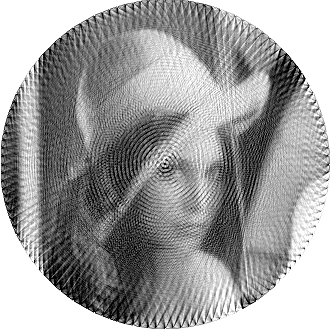
\includegraphics[width=\linewidth]{images/ls/ls_dense.png}
    \end{minipage}
    \begin{minipage}{0.2\linewidth}
        \centering
        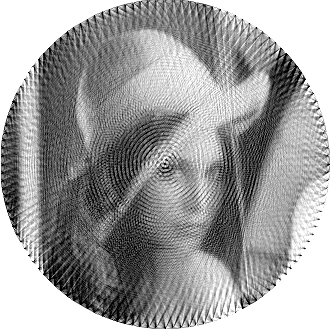
\includegraphics[width=\linewidth]{images/ls/ls_sparse.png}
    \end{minipage}
    \caption{Least Squares results for a system with 128 pegs with dense matrix representation (left) and sparse (right).}
    \label{fig:ls_output}
\end{figure}

\section{Linear Least Squares (LLS)}

To binarize the resulting vector \(x \in \left[-\infty, \infty\right]^{n}\), from the LS solver, a naive approach would be to select the top \(k\) highest values of \(x\) and choose the corresponding lines. To illustrate the limitations of this method, we present three configurations where the top 1000 lines are selected.

\begin{figure}[!htb]
    \centering
    \begin{minipage}{0.32\linewidth}
        \centering
        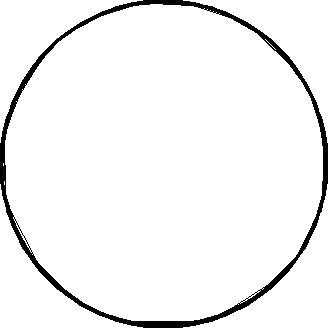
\includegraphics[width=\linewidth]{images/ls_binary/ls_rounding.png}
        \caption{Naive binarization of LS solver output.}
        \label{fig:ls_binary}
    \end{minipage}
    \hfill
    \begin{minipage}{0.32\linewidth}
        \centering
        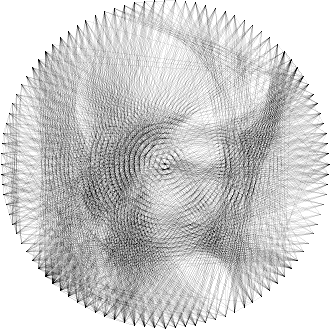
\includegraphics[width=\linewidth]{images/ls_binary/lls.png}
        \caption{Linear Least Squares (LLS) solver.}
        \label{fig:lls}
    \end{minipage}
    \hfill
    \begin{minipage}{0.32\linewidth}
        \centering
        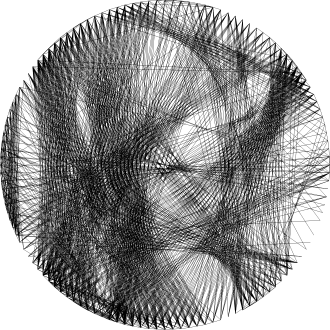
\includegraphics[width=\linewidth]{images/ls_binary/lls_binary.png}
        \caption{LLS solver with binarization and supersampling (\(\sigma=4\)).}
        \label{fig:lls_binary}
    \end{minipage}
\end{figure}

The figures above show the result of the standard LS solver (left), the Linear Least Squares (LLS) solver with box constraints \(x \in \left[0, 1\right]^{n}\) (center), and the LLS solver with both box constraints and binarization using supersampling with \(\sigma = 4\) (right). While the LLS solver requires approximately 30 seconds to compute, this added time is negligible within our scope.

The reason the LS solution (left) tends to select lines along the edge of the circle is due to the possibility of negative coefficients \(x_i\), which effectively allows it to \textit{subtract lines}, analogous to drawing with white string on the canvas. In its attempt to minimize reconstruction error, the solver chooses highly overlapping lines at the edge of the circle so it can subtract from them where needed.

\section{\texorpdfstring{Tuning N and $\sigma$}{Tuning N and sigma}}

The objective of this experiment is to determine the optimal number of pegs \(N\) and the block size \(\sigma\) for generating string art.

For the LS solver, the more we increase the number of pegs, the more the reconstructed image resembles the input image and the lower the residual becomes. However, increasing the number of pegs beyond \(256\) yields only marginal improvements that may not justify the added complexity.

\begin{figure}[H]
    \centering
    \begin{minipage}{0.75\linewidth}
        \centering
        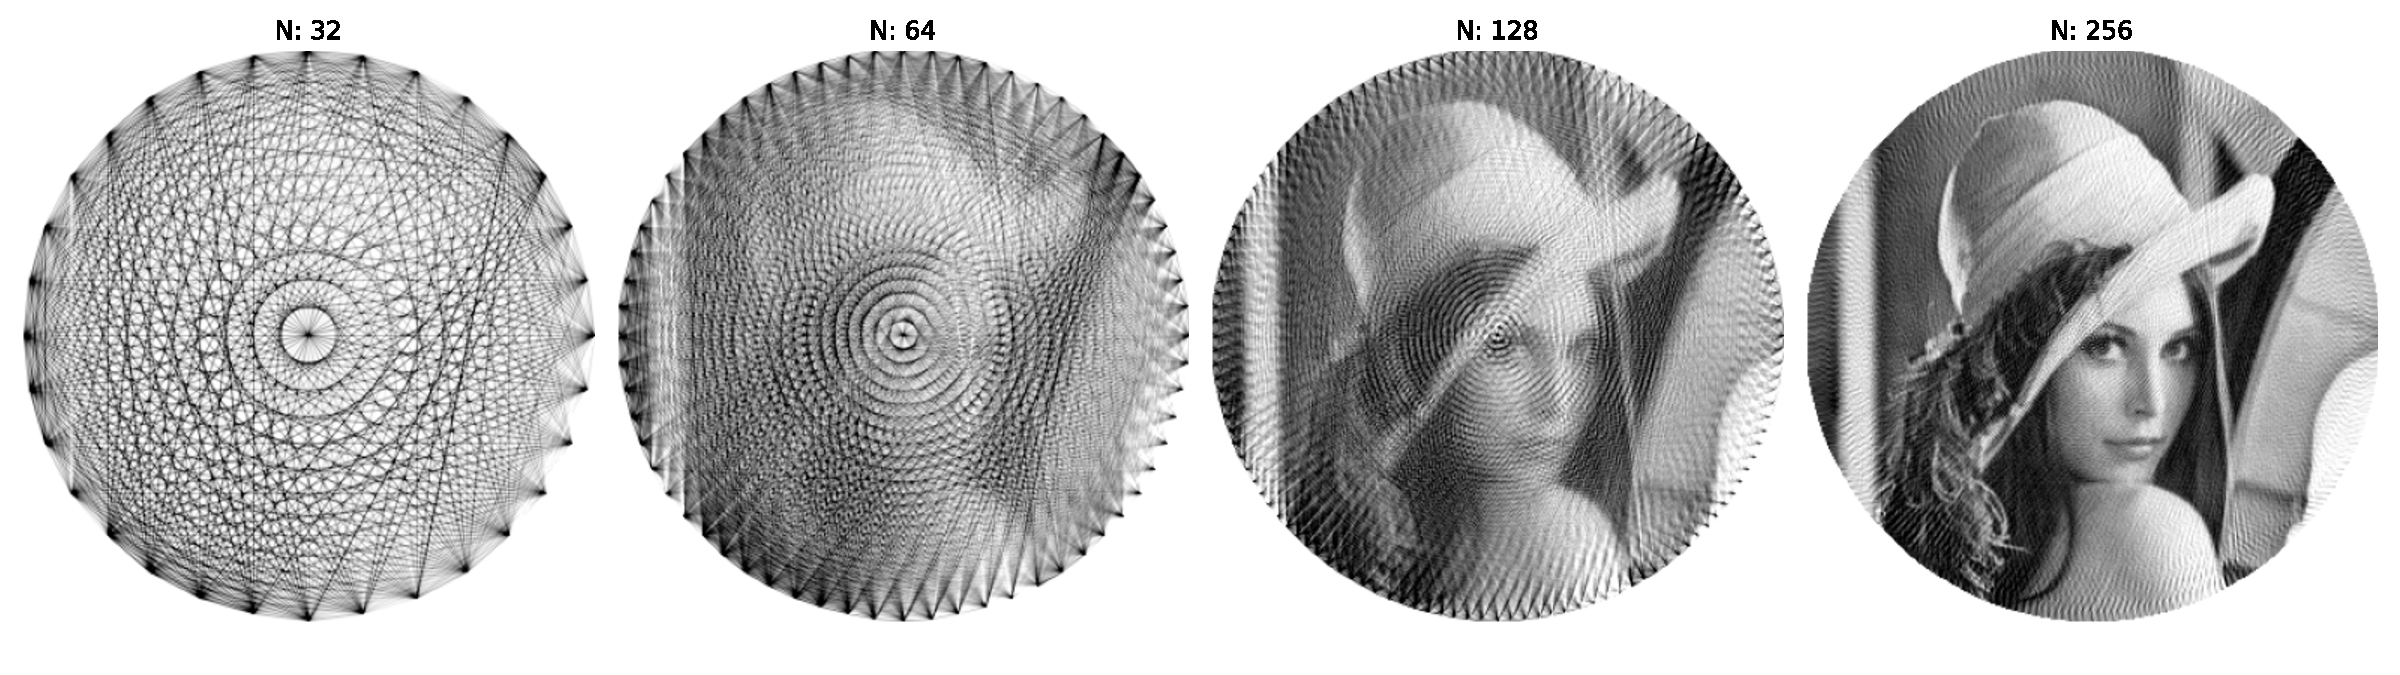
\includegraphics[width=\linewidth]{images/tuning/ls_images.pdf}
    \end{minipage}%
    \hfill
    \begin{minipage}{0.23\linewidth}
        \centering
        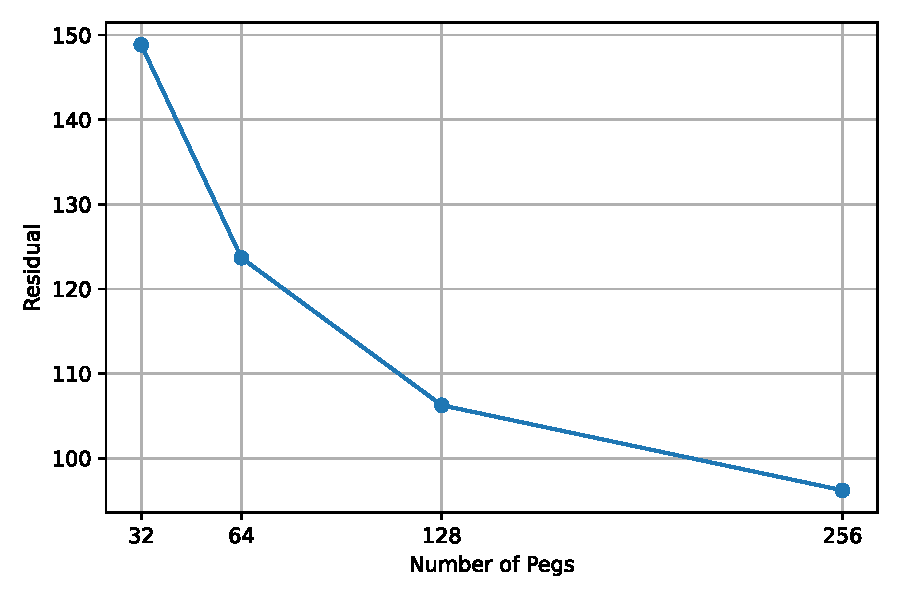
\includegraphics[width=\linewidth]{images/tuning/ls_residuals.pdf}
    \end{minipage}
    \caption{Comparative analysis and plot of residuals for results obtained using LS with different values of \(N\).}
    \label{fig:ls_n_tuning}
\end{figure}

To study the effect of block size \(\sigma\), we switch to a binary solver. This is essential because when we compute at a larger resolution as stated in Supersampling \ref{sec:supersampling}, white areas (thread gaps) grow more significantly than black areas (thread covered regions), affecting visual quality.

\begin{figure}[H]
    \centering
    \begin{subfigure}[t]{0.51\linewidth}
        \centering
        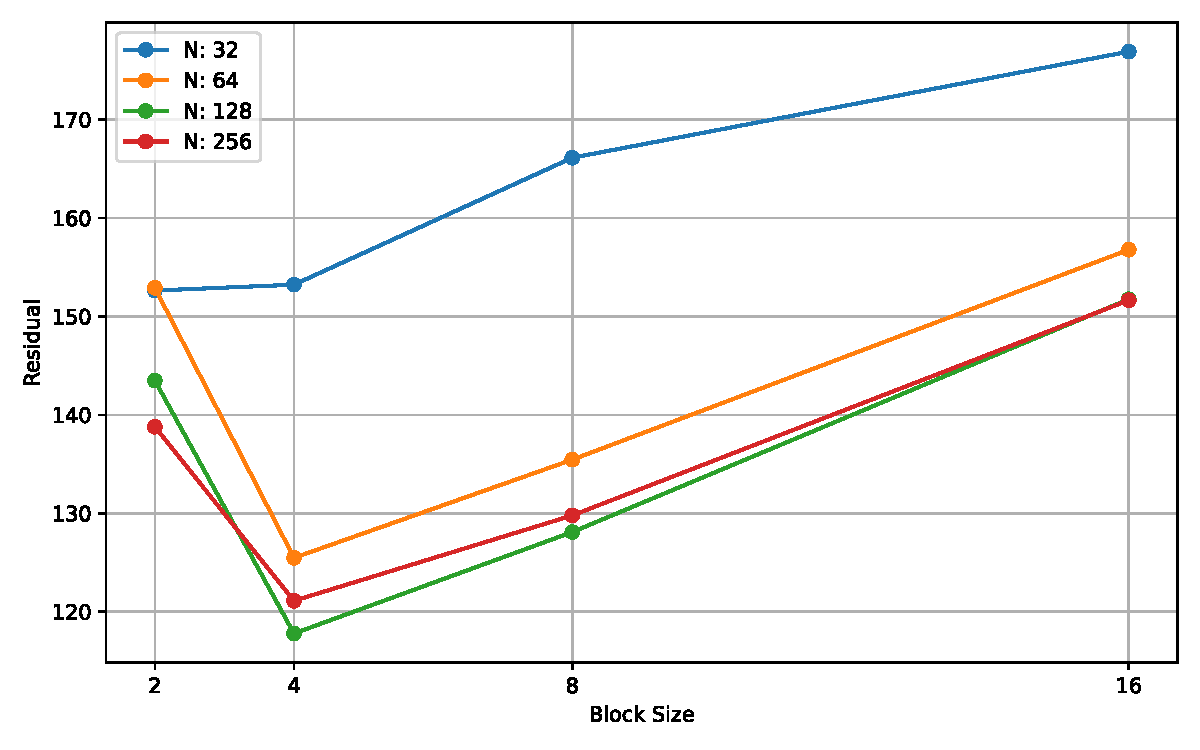
\includegraphics[width=\linewidth]{images/tuning/lls_residuals_by_pegs_and_block_size.pdf}
        \caption{}
    \end{subfigure}%
    \hfill
    \begin{subfigure}[t]{0.33\linewidth}
        \centering
        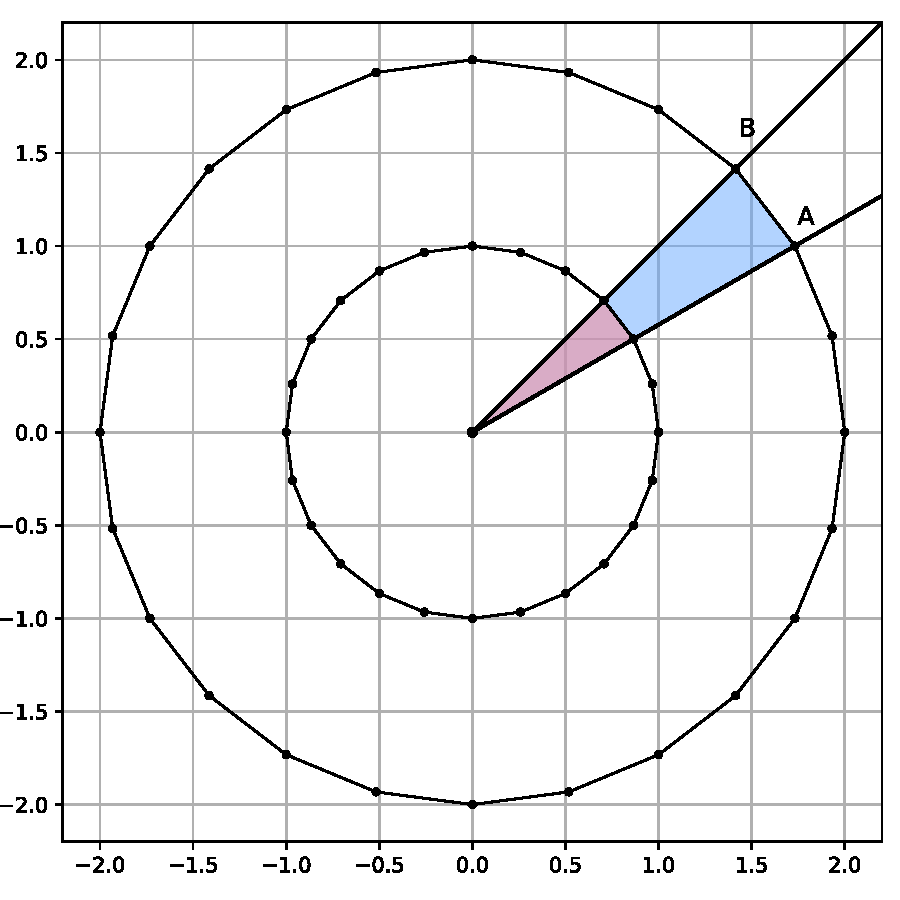
\includegraphics[width=\linewidth]{images/tuning/upsampling.pdf}
        \caption{}
        \label{fig:upsampling_A}
    \end{subfigure}
    \caption{(a) Residual error plotted against block size \(\sigma\). (b) Geometric interpretation of the upsampling process applied to matrix \(A\).}
    \label{fig:lss_residuals_by_pegs_ds}
\end{figure}

\begin{figure}[H]
    \centering
    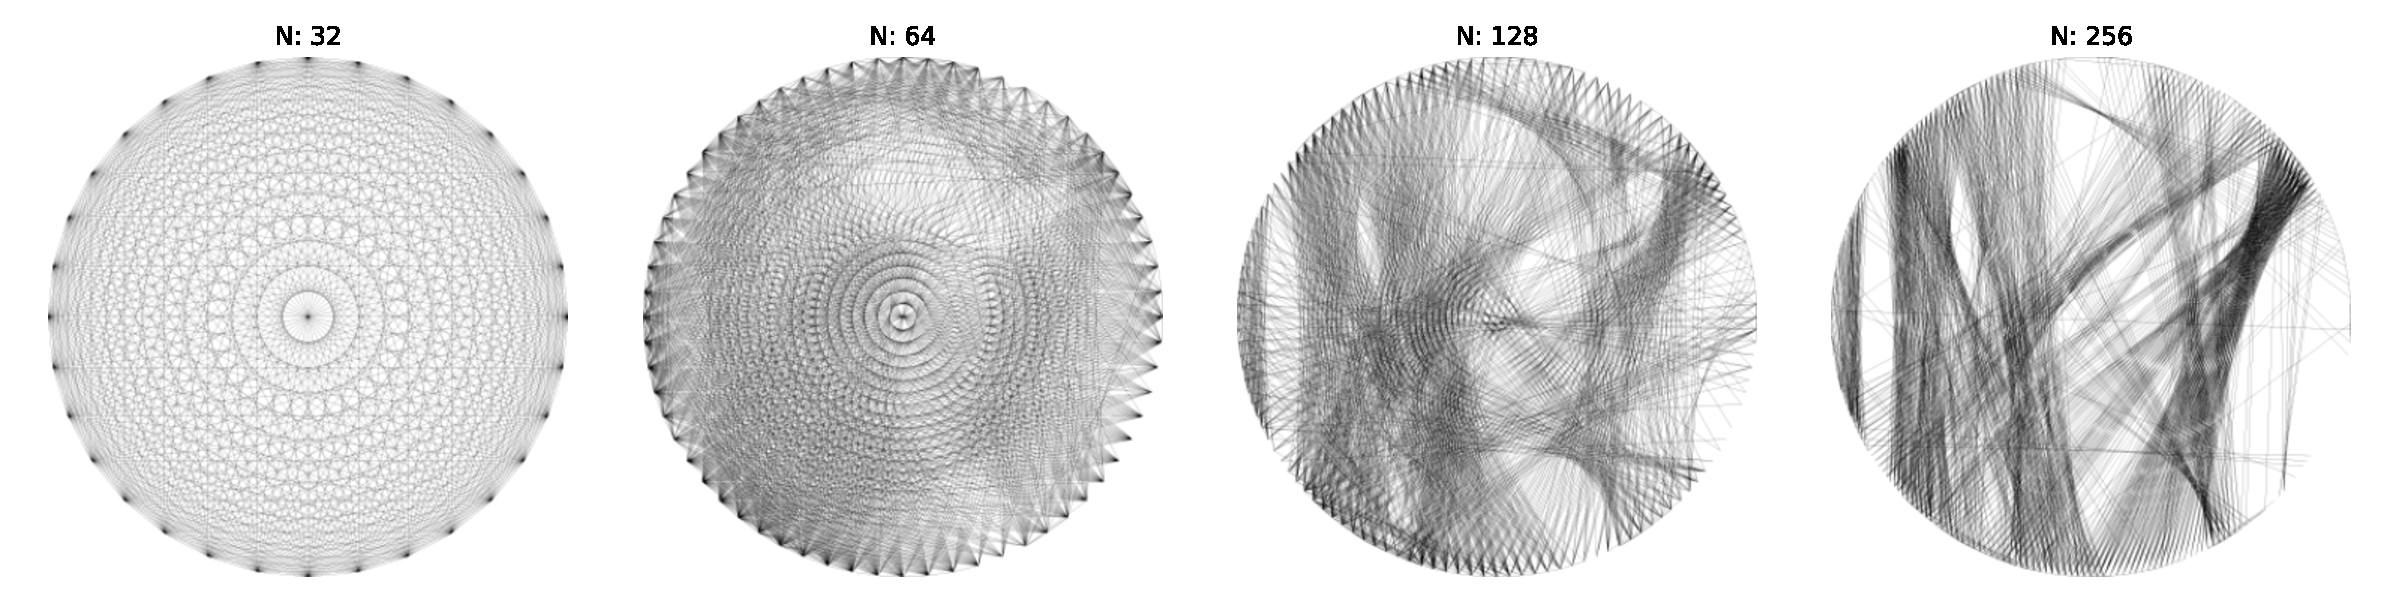
\includegraphics[width=\linewidth]{images/tuning/lls_column_2_as_row.pdf}
    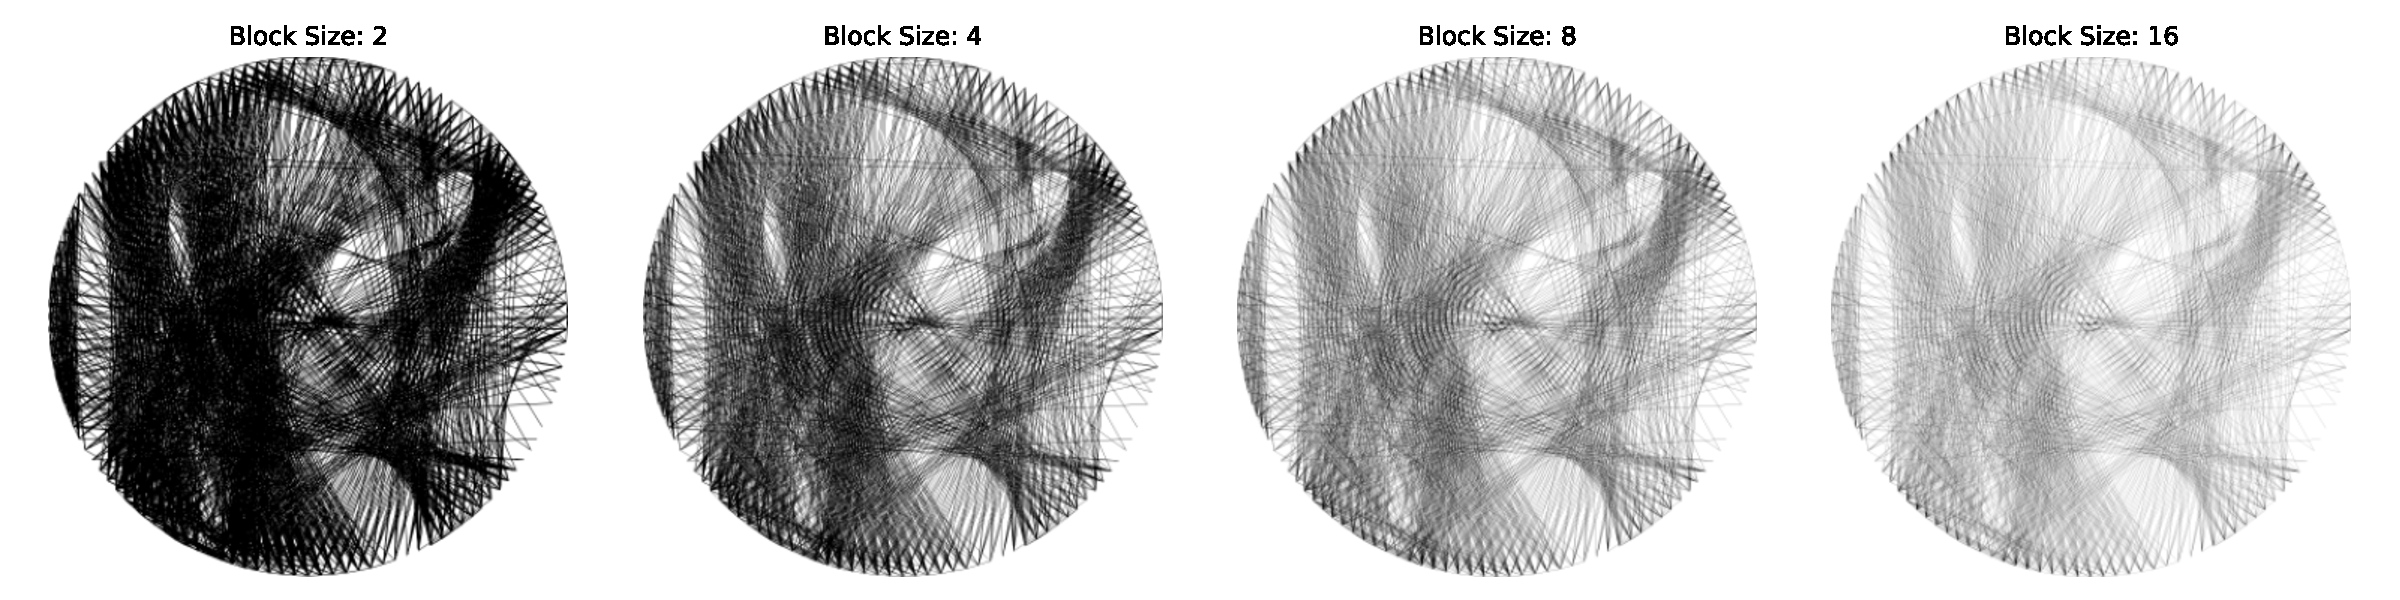
\includegraphics[width=\linewidth]{images/tuning/lls_row_2.pdf}
    \caption{Comparative analysis for varying \(N\) (top) and varying \(\sigma\) (bottom).}
    \label{fig:n_sigma_tuning}
\end{figure}

We can observe in Figure~\ref{fig:n_sigma_tuning} that the block size controls the thread thickness. Increasing it makes the image more transparent. Additionally, for this method, increasing \(N\) too much leads to incorrectly selecting the best lines (due to the naive solution). However, we shouldn't aim to use the maximum number of pegs, but rather choose the most optimal number for the given image. And that raises the question: \enquote{What is the best \(N\) for an image of size \(m \times m\)?}

As we can see in Figure~\ref{fig:upsampling_A}, the inner circle represents the original low-resolution matrix \(A\), while the outer circle corresponds to the upsampled matrix \(\bar{A}\). The white area between two adjacent pegs increases proportionally with the distance between those pegs. The idea is to plot the Manhattan distance and residual error for a selected set of \(N\) values, \(S = \{n_1, n_2, \ldots, n_t\}\), identify the optimal distance, and then use it to derive a formula for a general use. This leads us to:

\[
d = \frac{m}{2}\bigg(\left| \cos(\frac{2\pi}{N}) - 1 \right| + \left|  \sin(\frac{2\pi}{N})\right|\bigg)
\]

where \(d\) is the manhattan distance between two adjacent pegs (see Appendix~\ref{app:d} for a step-by-step derivation). 

\begin{figure}[H]
    \centering
    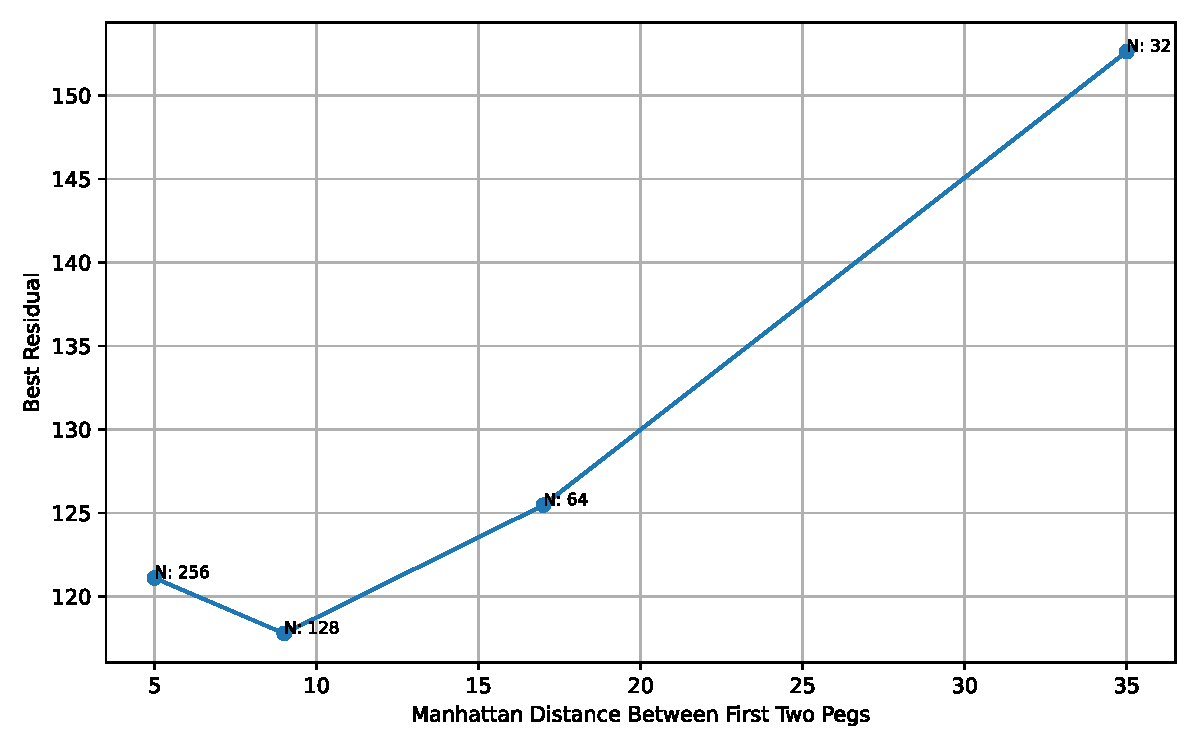
\includegraphics[width=0.5\linewidth]{images/tuning/lls_residuals_by_manhattan_distance.pdf}
    \caption{Best Residual vs. Peg-to-Peg Manhattan Distance.}
    \label{fig:residual_vs_manhattan}
\end{figure}

Plotting \(d\) alongside the residual error yields the figure above, from which we can observe that a Manhattan distance of approximately \(10\) provides the best result. This gives us the final formula:

\[
N = \underset{n \in S}{\arg\min} \left| d(n) - 10 \right|
\]

\section{Least Squares Regularized (LSR)}
\label{sec:lsr}

As explained in Convex Optimization \cite{convex-optimization}, we can cast our problem as a quadratic optimization problem. By using the CVXOPT Python package\footnote{For more details, see \href{https://cvxopt.org/}{CVXOPT: Python Software for Convex Optimization}}, we can integrate constraints and regularization terms. The equation we now need to minimize takes the form of a quadratic problem:

\begin{equation}
\label{eq:qp}
\min_{x} \frac{1}{2} x^TPx + q^Tx \quad \text{subject to } Gx \leq h
\end{equation}

where

\[
P = 2A^\top A, \quad q = -2A^\top b,
\]
\[
G = \begin{bmatrix}
-I \\
I
\end{bmatrix}, \quad
h = \begin{bmatrix}
\mathbf{0} \\
\mathbf{1}
\end{bmatrix}
\]

The constraint \( Gx \leq h \) enforces the box constraint: \(0 \leq x \leq 1\).

\subsubsection{Smooth Regularization}

We now implement the smooth regularization, given by the formula: \(4x(1-x)\). This regularizer promotes binary values by penalizing intermediate values in the range \(\left[0, 1\right]\). While this appears ideal, it has a significant drawback: the function is concave (see Figure~\ref{fig:regularization}), which violates the convexity required for our optimization problem.

To ensure the the matrix \(P\) stays positive semidefinite, a requirement for the CVXOPT solver, a safeguard is implemented by setting the regularization coefficient \(\lambda\) to the lowest eigenvalue of \(P\). Specifically, we ensure: \(\lambda \leq \frac{\lambda_{min}(P)}{8}\). The final modified objective:

\begin{equation}
\label{eq:qp_smooth}
\min_{x} \frac{1}{2} x^T(P - 8 \lambda I)x + (q + 4\lambda1)^Tx \quad \text{subject to } x \in [0,1]^n
\end{equation}

\begin{figure}[H]
    \centering
    \begin{minipage}{0.49\linewidth}
        \centering
        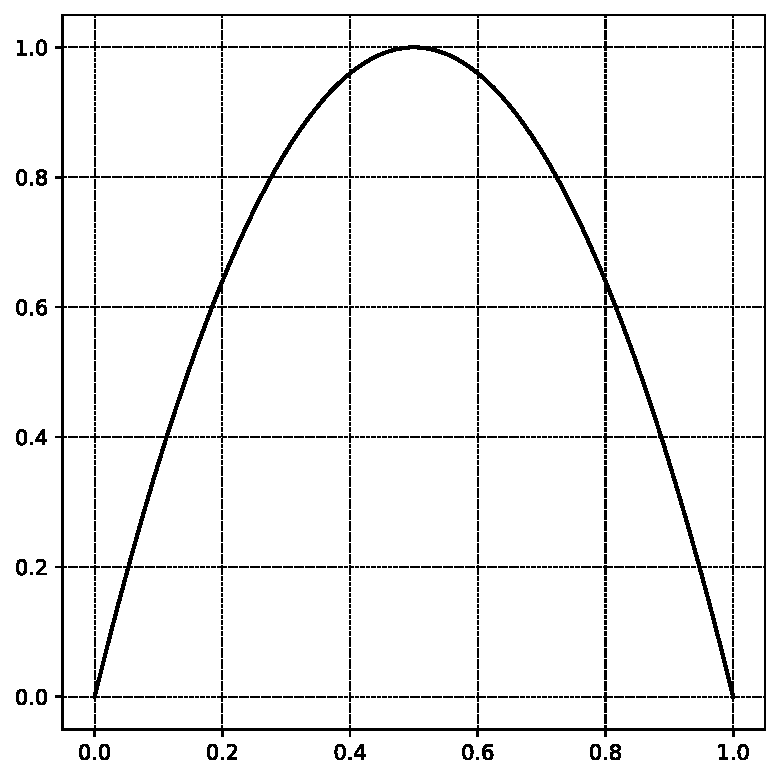
\includegraphics[width=\linewidth]{images/regularization/smooth_regularizer_graph.pdf}
    \end{minipage}%
    \begin{minipage}{0.49\linewidth}
        \centering
        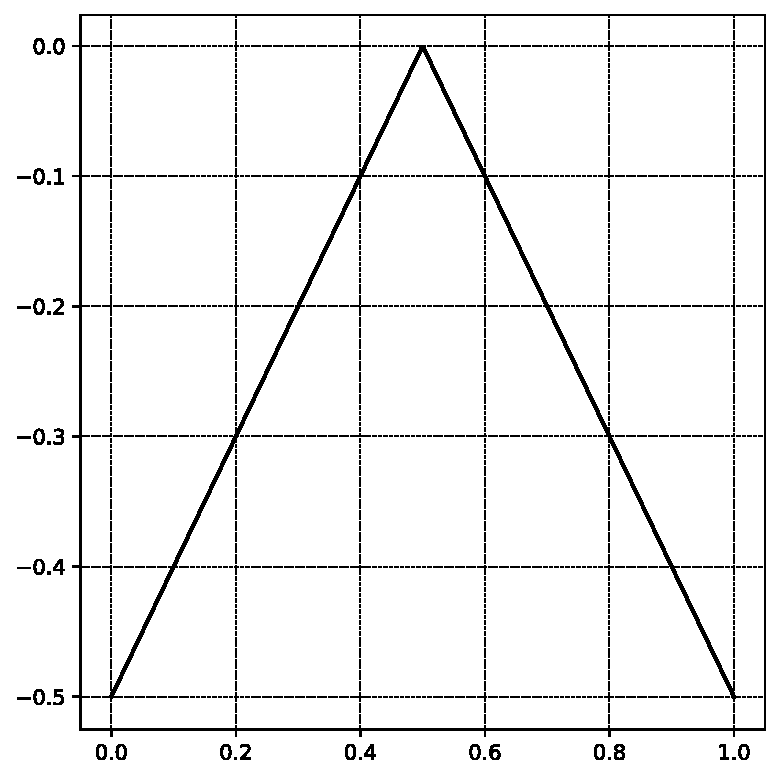
\includegraphics[width=\linewidth]{images/regularization/abs_regularizer_graph.pdf}
    \end{minipage}
    \caption{Smooth regularization graph (left) and Absolute regularization graph (right).}
    \label{fig:regularization}
\end{figure}

\subsubsection{Absolute Regularization}

We now introduce an alternative regularization term, given by the formula: \(1-2\left|x-0.5\right|\), which simplifies to \(-\left|x-0.5\right|\). The term \(\left|x-0.5\right|\) is convex, but its negation is concave. Including it in the objective breaks the convexity of the quadratic problem, making the problem non-convex.

To express the absolute value in a quadratic program, we introduce auxiliary variables: \(t_i \geq \left|x_i - 0.5\right|\) and optimize over: \(z = \left[x;t\right] \in \mathbb{R}^{2n}\). The modified objective and constraints:

\begin{equation}
\min_{x, t} \frac{1}{2} x^TPx + q^Tx - \lambda \sum_i{t_i} \quad \text{subject to } x \in [0,1]^n
\end{equation}

where
\[t \geq x - 0.5, \quad t \geq -x + 0.5\]

\begin{figure}[H]
    \centering
    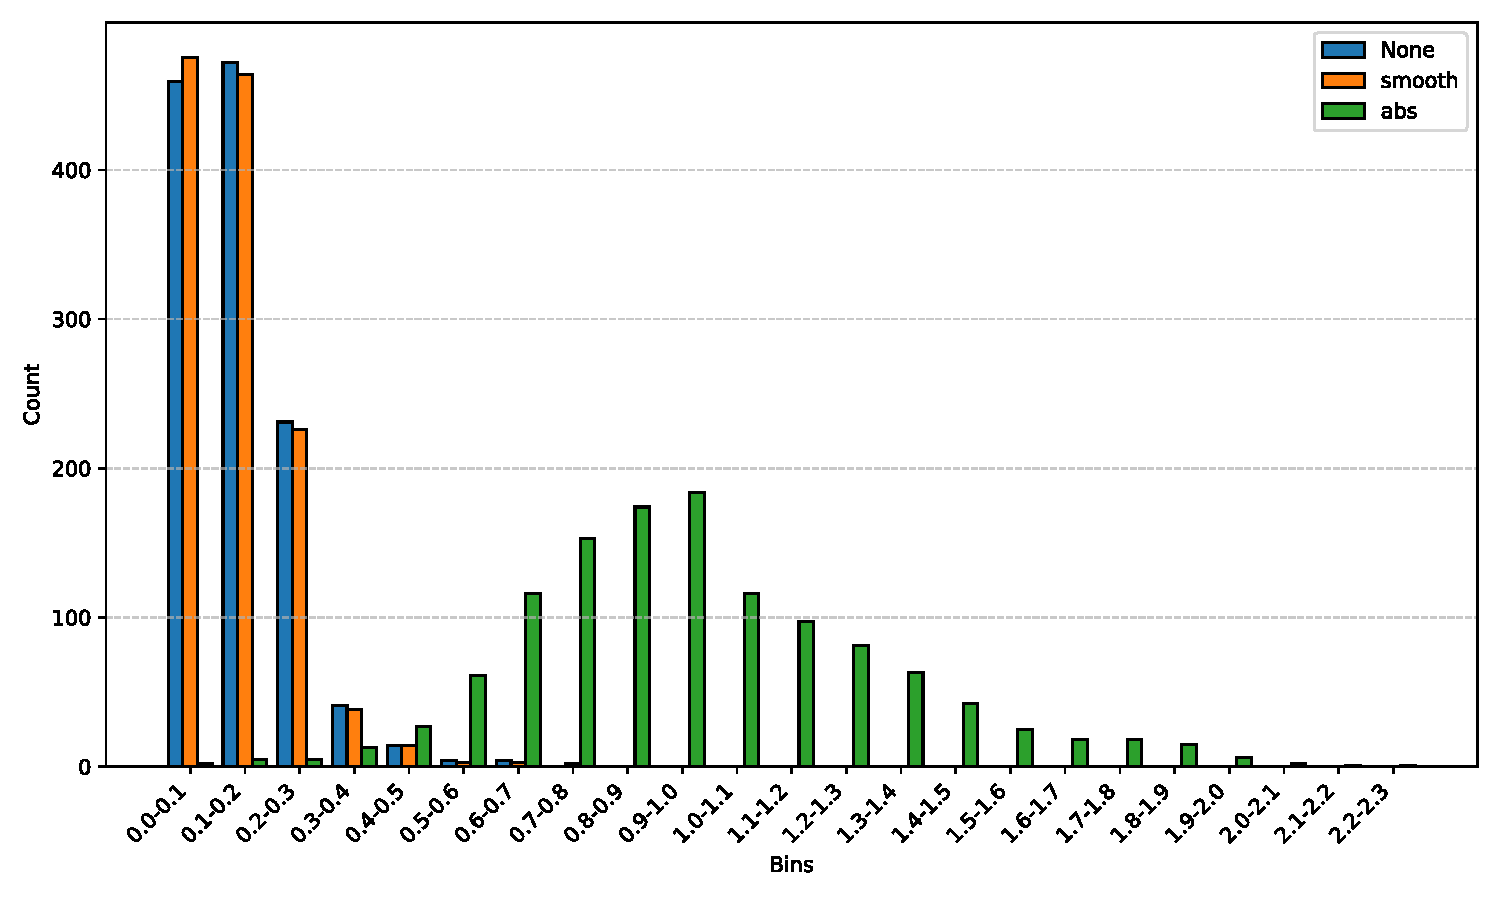
\includegraphics[width=\linewidth]{images/regularization/regularized_x_binned.pdf}
    \caption{Histogram illustrating the distribution of \(x\) coefficients with \(0.1\) bin span.}
    \label{fig:x_binned}
\end{figure}

The Smooth regularizer closely resembles the behavior of having no regularization, that is because the regularization strength \(\lambda\) is set very low to preserve the positive semidefinite property, which can be violated by stronger smoothness penalties. In contrast, the Absolute (abs) regularizer does succeed in pushing values towards \(1\), but it requires a very large regularization weight. However, this high value also causes violations of the imposed box constraints.

\begin{figure}[H]
    \centering
    \begin{minipage}{0.2\linewidth}
        \centering
        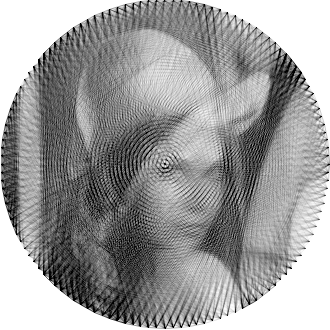
\includegraphics[width=\linewidth]{images/lsr/lsr_smooth.png}
    \end{minipage}
    \begin{minipage}{0.2\linewidth}
        \centering
        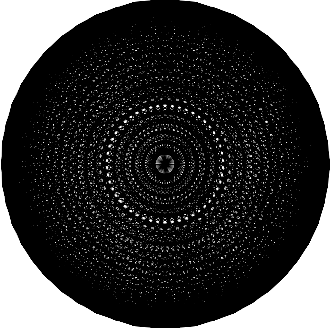
\includegraphics[width=\linewidth]{images/lsr/lsr_abs.png}
    \end{minipage}
    \caption{Least Squares Regularized results for a system with 128 pegs with smooth regularization (left) and absolute (right).}
    \label{fig:lsr_output}
\end{figure}

\section{Binary Projection Least Squares (BPLS)}

In Section~\ref{sec:lsr}, it was noted that introducing a binary enforcing regularization term can break the convexity of the optimization problem. To address this, a new approach was proposed: instead of adding the regularization term explicitly to the objective, we incorporate its effect directly into the cost matrix before solving the system. This preserves convexity while still encouraging binary-like solutions through adaptive weighting.

We will now introduce the following vector \(w\). This vector forms the diagonal of a regularization matrix \(W = diag(w)\), which is used to modify the original quadratic cost matrix \(P\). The updated regularized problem becomes:

\begin{equation}
\label{eq:bpls}
\min_{x} \frac{1}{2} x^T(P + \lambda W)x + q^Tx \text{ subject to } x \in [0,1]^n
\end{equation}

The first iteration begins with \(W = I\), and we update the weights at step \(i\) using the formula \(w_i = x_{i-1}(1-x_{i-1}) + \epsilon\). We solve the problem described by Equation~\ref{eq:bpls}, then select the the top \(k\) values from \(x\) and fix those to \(1\). Next, we adjust the problem by calculating the contributions of the selected lines: \(A_1 1\), where \(A_1\) is the subset of lines corresponding to the selected indices in this iteration. We subtract this from \(b\): \(\bar{b} = b - A_1 1\). This process is repeated with the updated \(\bar{b}\) until the error stops decreasing or a maximum number of iterations is reached.

\begin{figure}[H]
    \centering
    \begin{minipage}{0.2\linewidth}
        \centering
        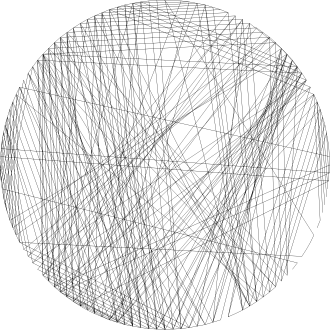
\includegraphics[width=\linewidth]{images/bpls/bpls_earlystopping.png}
    \end{minipage}
    \begin{minipage}{0.2\linewidth}
        \centering
        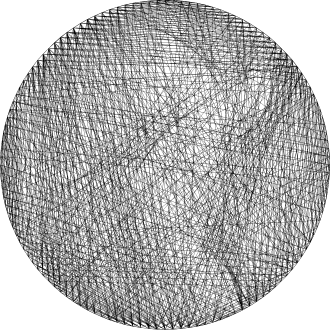
\includegraphics[width=\linewidth]{images/bpls/bpls.png}
    \end{minipage}
    \caption{Binary Projection Least Squares results for a system with 128 pegs, \(k=10\) and \(\lambda=100\): with early stopping (left) and without early stopping, using a maximum of 90 iterations (right).}
    \label{fig:bpls_output}
\end{figure}

\section{Matching Pursuit (MP)}

Matching Pursuit is a greedy algorithm used to approximate a signal by selecting dictionary vectors one by one. In our case, the signal is the \(b\) vector, and the dictionary vectors are the column vectors of the matrix \(A\).

Below, we present two methods of matching pursuit: Greedy Matching Pursuit and Orthogonal Matching Pursuit (OMP). Both methods will be analyzed using the selection of 1000 lines, with experiments conducted using both real valued and binary coefficients.

\subsection{Greedy}

The greedy method consists of selecting the line that reduces the residual error the most at each step. Once a line is chosen, the decision is irreversible. This method is computationally intensive on a typical personal use PC. To address this, we introduce two heuristics to reduce the number of candidate lines evaluated at each step: random, where we randomly select \(l\) candidate lines, in our experiments \(l=100\) provides a good trade-off between accuracy and computation time, and dot-product, where we compute the scalar product \(A^Tb\) and select the top \(l\) based on this score. See Appendix~\ref{app:greedy} for the pseudocode of this algorithm.

\subsection{Orthogonal Matching Pursuit (OMP)}

The Orthogonal Matching Pursuit (OMP) method is very similar to the Greedy one, following the same kind of iterative process based on selecting the line that reduces the error the most. In contrast, OMP updates the residual \(b\) (initially the input image) by subtracting the projection of the selected line. This ensures that the residual remains orthogonal to all lines selected so far. See Appendix~\ref{app:omp} for the pseudocode of this algorithm.

\begin{figure}[H]
    \centering
    \begin{minipage}{0.2\linewidth}
        \centering
        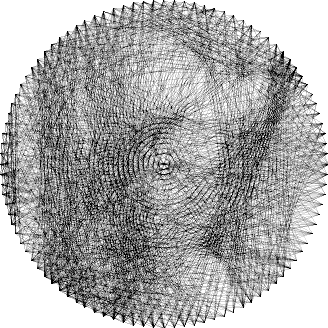
\includegraphics[width=\linewidth]{images/mp/greedy_random.png}
    \end{minipage}
    \begin{minipage}{0.2\linewidth}
        \centering
        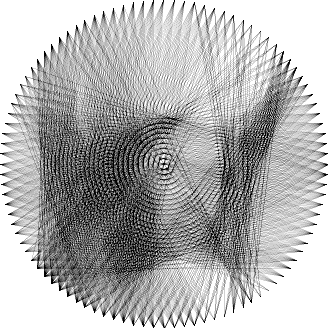
\includegraphics[width=\linewidth]{images/mp/greedy_dotproduct.png}
    \end{minipage}
    \begin{minipage}{0.2\linewidth}
        \centering
        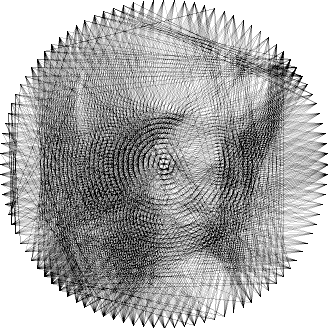
\includegraphics[width=\linewidth]{images/mp/omp.png}
    \end{minipage}
    \caption{Matching Pursuit results for a system with 128 pegs and 1000 selected lines, using real valued \(x\) coefficients and without early stopping. The methods, in order, are: Greedy (random heuristic), Greedy (dot-product heuristic), and Orthogonal Matching Pursuit.}
    \label{fig:mp_outputs}
\end{figure}

\begin{figure}[H]
    \centering
    \begin{minipage}{0.2\linewidth}
        \centering
        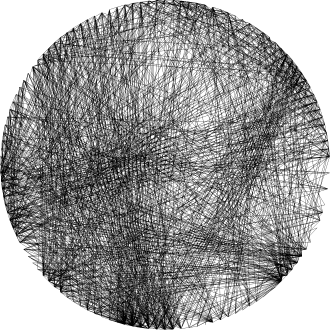
\includegraphics[width=\linewidth]{images/mp_binary/greedy_random_binary.png}
    \end{minipage}
    \begin{minipage}{0.2\linewidth}
        \centering
        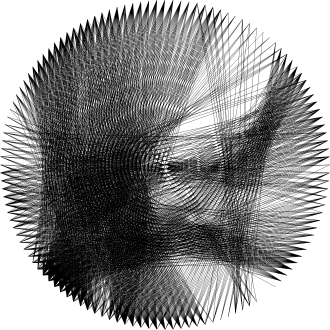
\includegraphics[width=\linewidth]{images/mp_binary/greedy_dot-product_binary.png}
    \end{minipage}
    \begin{minipage}{0.2\linewidth}
        \centering
        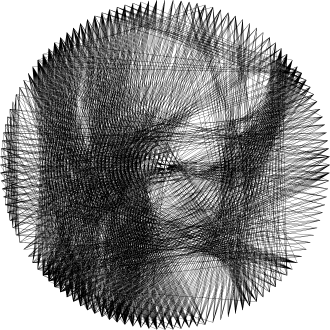
\includegraphics[width=\linewidth]{images/mp_binary/omp_binary.png}
    \end{minipage}
    \caption{Matching Pursuit results for a system with 128 pegs and 1000 selected lines, using binary valued \(x\) coefficients with supersampling and without early stopping. The methods, in order, are: Greedy (random heuristic), Greedy (dot-product heuristic), and Orthogonal Matching Pursuit.}
    \label{fig:mp_binary_outputs}
\end{figure}

\section{Radon Transform}

The Radon Transform maps an image \(f(x,y)\) to a collection of line integrals through \(f(x,y)\). We can express it as follows: \(\text{Let } L(\theta, s) = \{(x, y) \in \mathbb{R}^2 : x\cos\theta + y\sin\theta = s\} \text{ be the line integral}\), where \(\theta \in \left[0, \pi\right)\) is the angle the line makes with the x-axis and \(s \in \left[ -r, r\right]\), is the signed perpendicular distance from the origin to the line, and \(r\)  is the radius of the inscribed circle within the image. Then, we define:

\begin{equation}  
R(\theta, s) = \int_{L(\theta, s)} f(x, y)ds
\end{equation}

\begin{figure}[H]
    \centering
    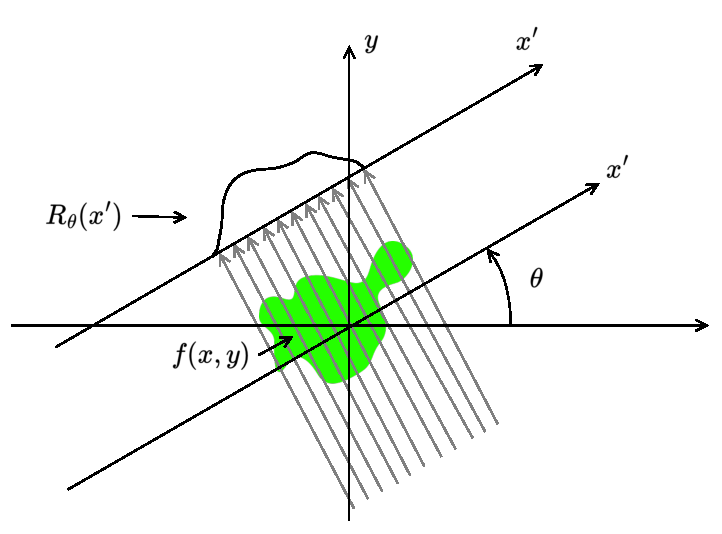
\includegraphics[width=0.6\linewidth]{images/radon.pdf}
    \caption{Radon Transform Illustration.}
    \label{fig:radon_illustration}
\end{figure}

Using the illustration above, we can think of the Radon transform like a laser beam that scans through the image. At each angle and distance, the laser measures how much of the image’s content (or density) it passes through. By collecting these measurements from different angles and positions, we get a full set of line integrals that represent the image from many perspectives.

In our string art problem, the lines we draw can also be described using the same notation with \(\theta\) and \(s\) as above. This means another way to solve the string art problem is to compute the Radon Transform of all possible lines across our circle and select the line with the highest value to draw next. \textbf{Important}: each line’s projection should be normalized by dividing by its length. Otherwise, the algorithm would favor longer lines over shorter, darker ones.

After selecting a line, we need to subtract its contribution from the sinogram, and also from all other lines. Because lines intersect and depend on each other, this means the basis is not orthogonal. We continue this process as long as the error decreases by more than a minimum delta, and we use a customizable patience factor to control when to stop.

We implemented a custom Radon Transform because we can take advantage of the constraints in the string art problem. Instead of representing the sinogram as a matrix indexed by \(\theta\) and \(s\), it’s stored as a list where each index \(i\) corresponds to the density of line \(i\). We select the line with the highest value, remove it from the list, and then update all other lines by removing the pixels that intersect with the chosen line. This keeps the space orthogonal. This update step has a time complexity of \(O(N^2)\), resulting in a final algorithm complexity of \(O(N^4)\).

\begin{figure}[H]
    \centering
    \begin{minipage}{0.2\linewidth}
        \centering
        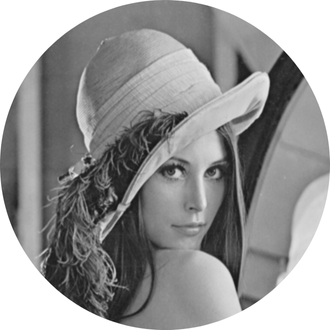
\includegraphics[width=\linewidth]{images/radon/lena_bw.png}
    \end{minipage}
    \begin{minipage}{0.2\linewidth}
        \centering
        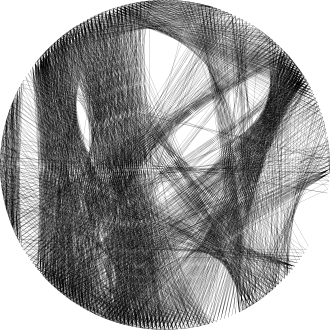
\includegraphics[width=\linewidth]{images/radon/lena_radon.png}
    \end{minipage}
    \begin{minipage}{0.2\linewidth}
        \centering
        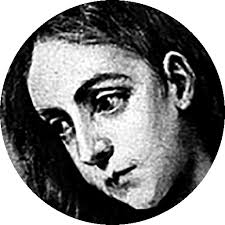
\includegraphics[width=\linewidth]{images/radon/mary.png}
    \end{minipage}
    \begin{minipage}{0.2\linewidth}
        \centering
        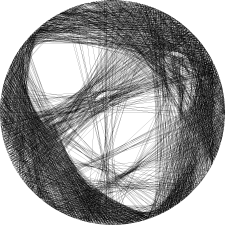
\includegraphics[width=\linewidth]{images/radon/mary_radon.png}
    \end{minipage}
    \caption{Radon Transform results for a system with 256 pegs and early stopping mechanism.}
    \label{fig:radon_output}
\end{figure}

\subsubsection{Enhancing the Radon Transform Method}
\label{sec:radon_improvements}

While standard Radon implementations (like those in scikit-learn) run in \(O(NlogN)\), compared to the \(O(N^2)\) complexity of our algorithm, our approach avoids the overhead of computing the sinogram of the intersection between two lines and then subtracting it from all other lines. Although this may sound straightforward, it is actually more complex than implementing manual projection calculations and the orthogonal projection update.

Another way to speed up our Radon Transform is to update only the lines that intersect the chosen line, limiting updates to the number of intersections instead of all lines. Of course, the initial computation of the Radon Transform still has a time complexity of \(O(N^2)\). However, when subtracting the contribution of the chosen line, the update step now becomes more efficient, with time complexity \(O(k)\), where \(k\) is the maximum number of possible intersections across all lines. 

This raises an important question: \textit{Which is the worst line to draw?}, or more formally: \textit{Which line causes the most intersections if drawn?} As a result, the final time complexity becomes \(O(N^2k)\).

To answer the question above, intersections occur when the selected line partitions the circle into two regions, and other lines attempt to connect points from opposite sides of this partition. Any such line will necessarily intersect the dividing line. Intuitively, the worst-case dividing line is the one that perfectly splits the circle into two equal halves. In this case, each of the \(\frac{N}{2}\) pegs on one side can potentially connect to each of the \(\frac{N}{2}\) pegs on the other side, resulting in a maximum of \((\frac{N}{2})^2 = \frac{N^2}{4}\) intersections. This remains to be formally proven.